\documentclass{acm_proc_article-sp}
\usepackage[utf8]{inputenc}

\renewcommand{\paragraph}[1]{\vskip 6pt\noindent\textbf{#1 }}
\usepackage{hyperref}
\usepackage{graphicx}
\usepackage{url}

\title{Impacto do número de cores e arquitetura de CPU no desempenho do
emulador RPCS3}


% Add imagehandling

\numberofauthors{2}
\author{
\alignauthor Victor Furusho Vally \\
        \affaddr{Universidade Federal do Rio Grande do Sul}\\
       \email{}
\and \alignauthor Erick Schultz Ceresa \\
        \affaddr{Universidade Federal do Rio Grande do Sul}\\
       \email{}
\and }

\date{}

%Remove copyright shit
\permission{}
\conferenceinfo{} {}
\CopyrightYear{}
\crdata{}


% tightlist command for lists without linebreak
\providecommand{\tightlist}{%
  \setlength{\itemsep}{0pt}\setlength{\parskip}{0pt}}




\begin{document}


\maketitle

\begin{abstract}
This is the abstract.

It consists of two paragraphs.
\end{abstract}

\section{Introdução}\label{introduuxe7uxe3o}

A emulação de hardware de arquiteturas diversas é um grande desafio na
computação, mas um desafio que as comunidades open source rotinamente
aceitam, principalmente para consoles de jogos, com o intuito de manter
a biblioteca de software desses consoles preservada.

O RPCS3 é um desses emuladores. A emulação do Playstation 3 é um desafio
maior do que o comum para seus desenvolvedores, já que o Playstation 3
possui hardware exótico em sua arquitetura e difícil de mapear para
arquiteturas atuais como x86\_64.

O Playstation 3 oferece vários componentes em operação paralela, os
principais sendo: 8 unidades de processamento SIMD com alta vasão
chamadas SPEs ou Synergistic Processing Elements, dentro das quais 6
podem ser utilizadas por software, uma é reservada para o OS e uma é
desativada; um ring buffer que alimentar as SPEs com instruções e dados,
chamado Element Interconnect Bus; e por fim um processador principal
chamado de PPE, ou Power Processing Element. Todos com seu próprio cache
e instruções.

É fácil de perceber que implementar um sistema compatível em software é
uma tarefa complicada. Não é apenas necessário que a arquitetura do
emulador seja sólida, mas que o hardware host seja utilizado
eficientemente para que a emulação ocorra em velocidades interagíveis. O
maior obstáculo para a eficiência da emulação do Playstation 3 é o
paralelismo, o que é espelhado na arquiteturo do console: no mínimo é
necessário que ocorram 7 operações em paralelo, sem contar os
componentes que cercam o complexo principal do processador e os
segmentos do ring buffer. Por consequência, toda a demanda cai sobre a
CPU do sistema host, o que é consolidado nos requisitos do RPCS3: uma
grande disparidade entre o tier de performance da CPU comparada a CPU.

Visamos explorar a relação entre o número de núcleos do processador host
e a performance de emulação no emulador RPCS3. Utilizando um dos jogos
mais exigentes no hardware do Playstation 3, The Last of Us, utilizando
o tempo entre a geração de cada quadro, ou frametime, para contrastar a
performance entre 6, 8 e 12 núcleos do mesmo processador. Também
comparamos duas arquiteturas de processador com 6 núcleos.

\begin{figure}[t]
\centering
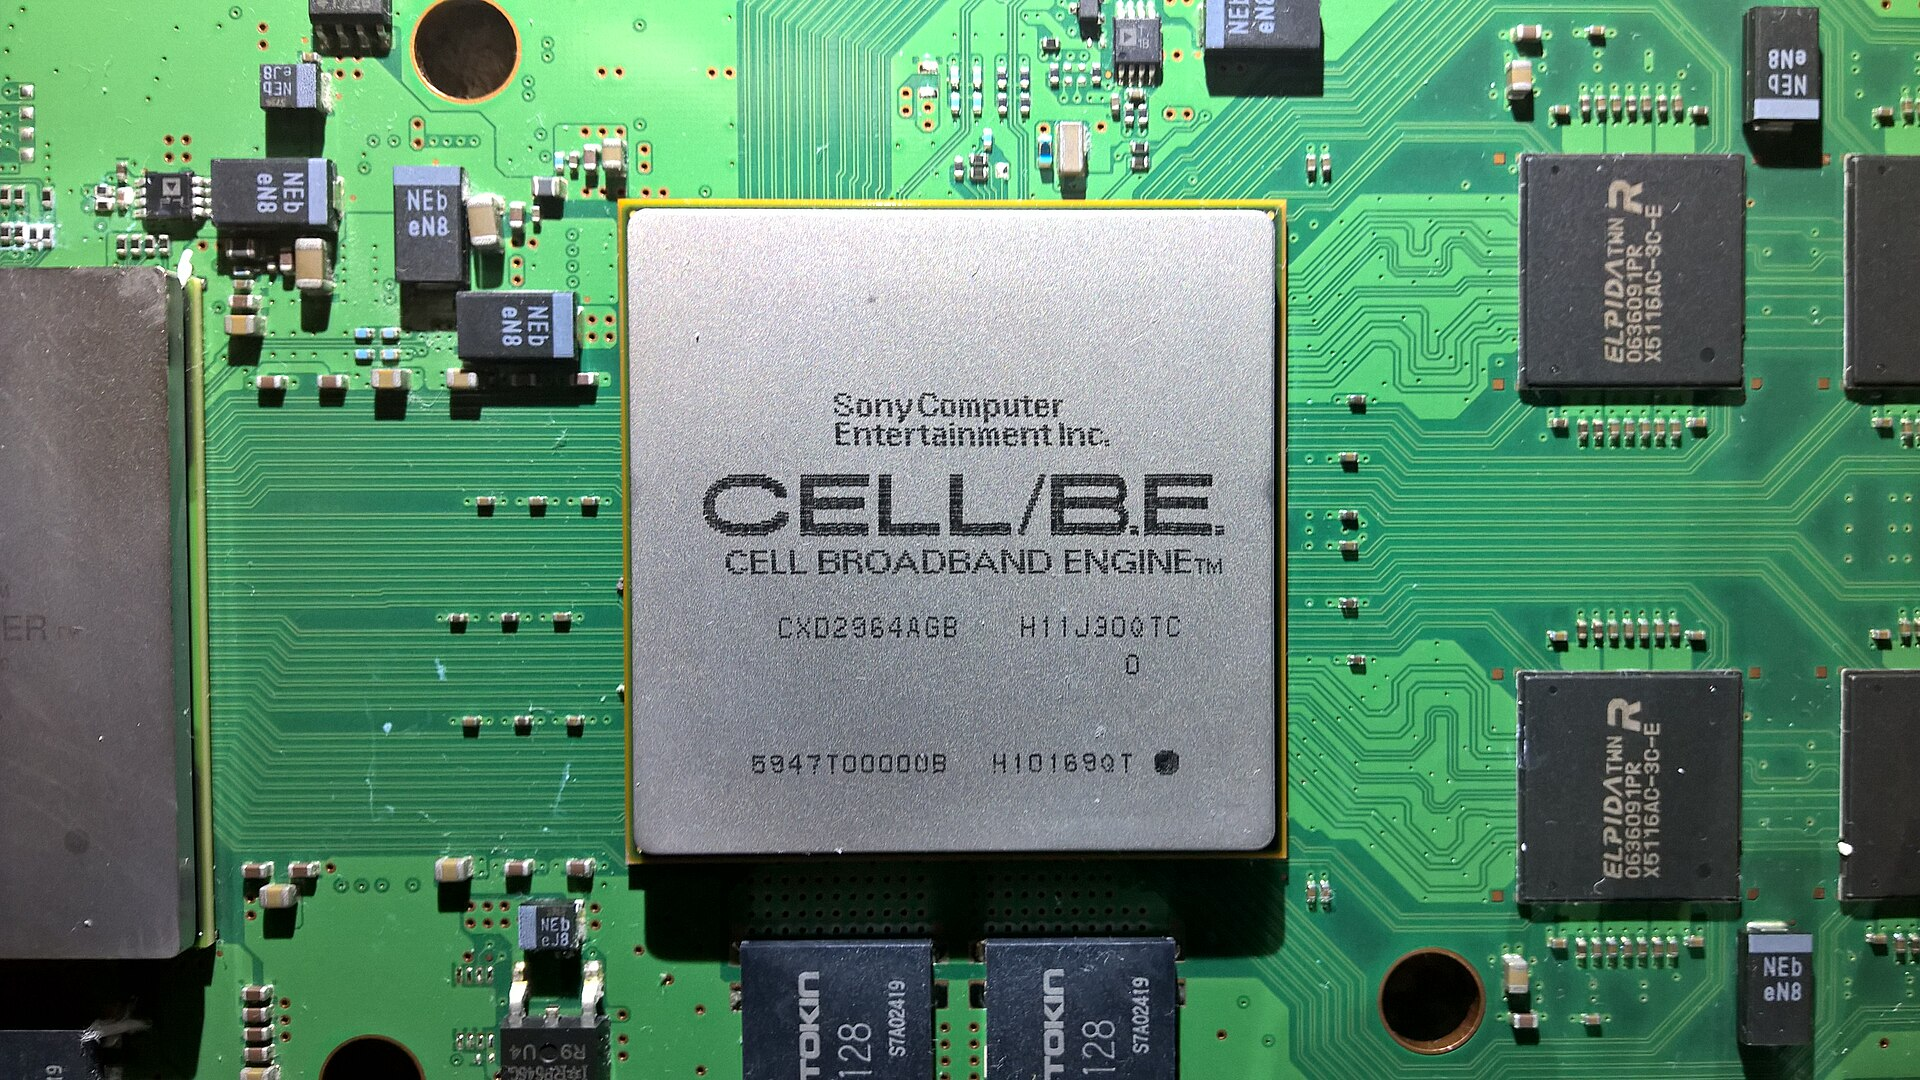
\includegraphics[width=0.9\linewidth]{images/cell.jpg}
\caption{Processador CELL}
\label{fig:cell}
\end{figure}

\section{Avaliação}\label{avaliauxe7uxe3o}

O objetivo desta avaliação é quantificar o impacto do número de núcleos
do processador hospedeiro e da arquitetura da CPU no desempenho do
emulador RPCS3, com foco em variações de frametime sob condições
controladas de execução.

\subsubsection{Ambiente experimental}\label{ambiente-experimental}

Os experimentos foram conduzidos em duas plataformas computacionais
distintas. A primeira utiliza um processador AMD Ryzen 9 9900X, com 12
núcleos e 24 threads, frequência base de 4,4 GHz e frequência máxima de
5,6 GHz, acompanhado de uma GPU AMD Radeon RX 7800 XT. A segunda utiliza
um processador Intel Core i5-10400F, com 6 núcleos e 12 threads,
frequência base de 2,9 GHz e frequência máxima de 4,3 GHz e uma GPU RTX
2060.

Ambas as máquinas executam o sistema operacional NixOS. A compilação do
RPCS3 e seu ambiente de execução foram feitas por meio do gerenciador de
pacotes Nix, garantindo que ambas as plataformas utilizassem versões
idênticas de bibliotecas, dependências e opções de compilação. Dessa
forma, buscou-se minimizar diferenças de software entre os sistemas,
permitindo que as variações observadas fossem atribuídas
predominantemente às características do hardware.

Foram criados dois scripts para simplificação do setup do ambientes. O
primeiro é o script build.sh, que baixa e compila o fork instrumentado
do RPCS3. O segundo é run.sh, que carrega as dependências necessárias e
inicializa o emulador.

\subsubsection{Carga de trabalho}\label{carga-de-trabalho}

Como carga de trabalho, foi utilizado o jogo \emph{The Last of Us},
escolhido por sua alta exigência computacional no contexto do
PlayStation 3. Para reduzir variabilidade associada a cenas dinâmicas,
dois estados distintos do jogo foram selecionados a partir de saves
específicos. Em cada estado, o personagem permaneceu inativo durante
toda a coleta de dados, evitando interferência de inputs de usuário.

Os dois cenários selecionados representam uma carga de trabalho intensa
para a CPU, com múltiplos persoágens na tela ao mesmo tempo.

\begin{figure}[t]
\centering
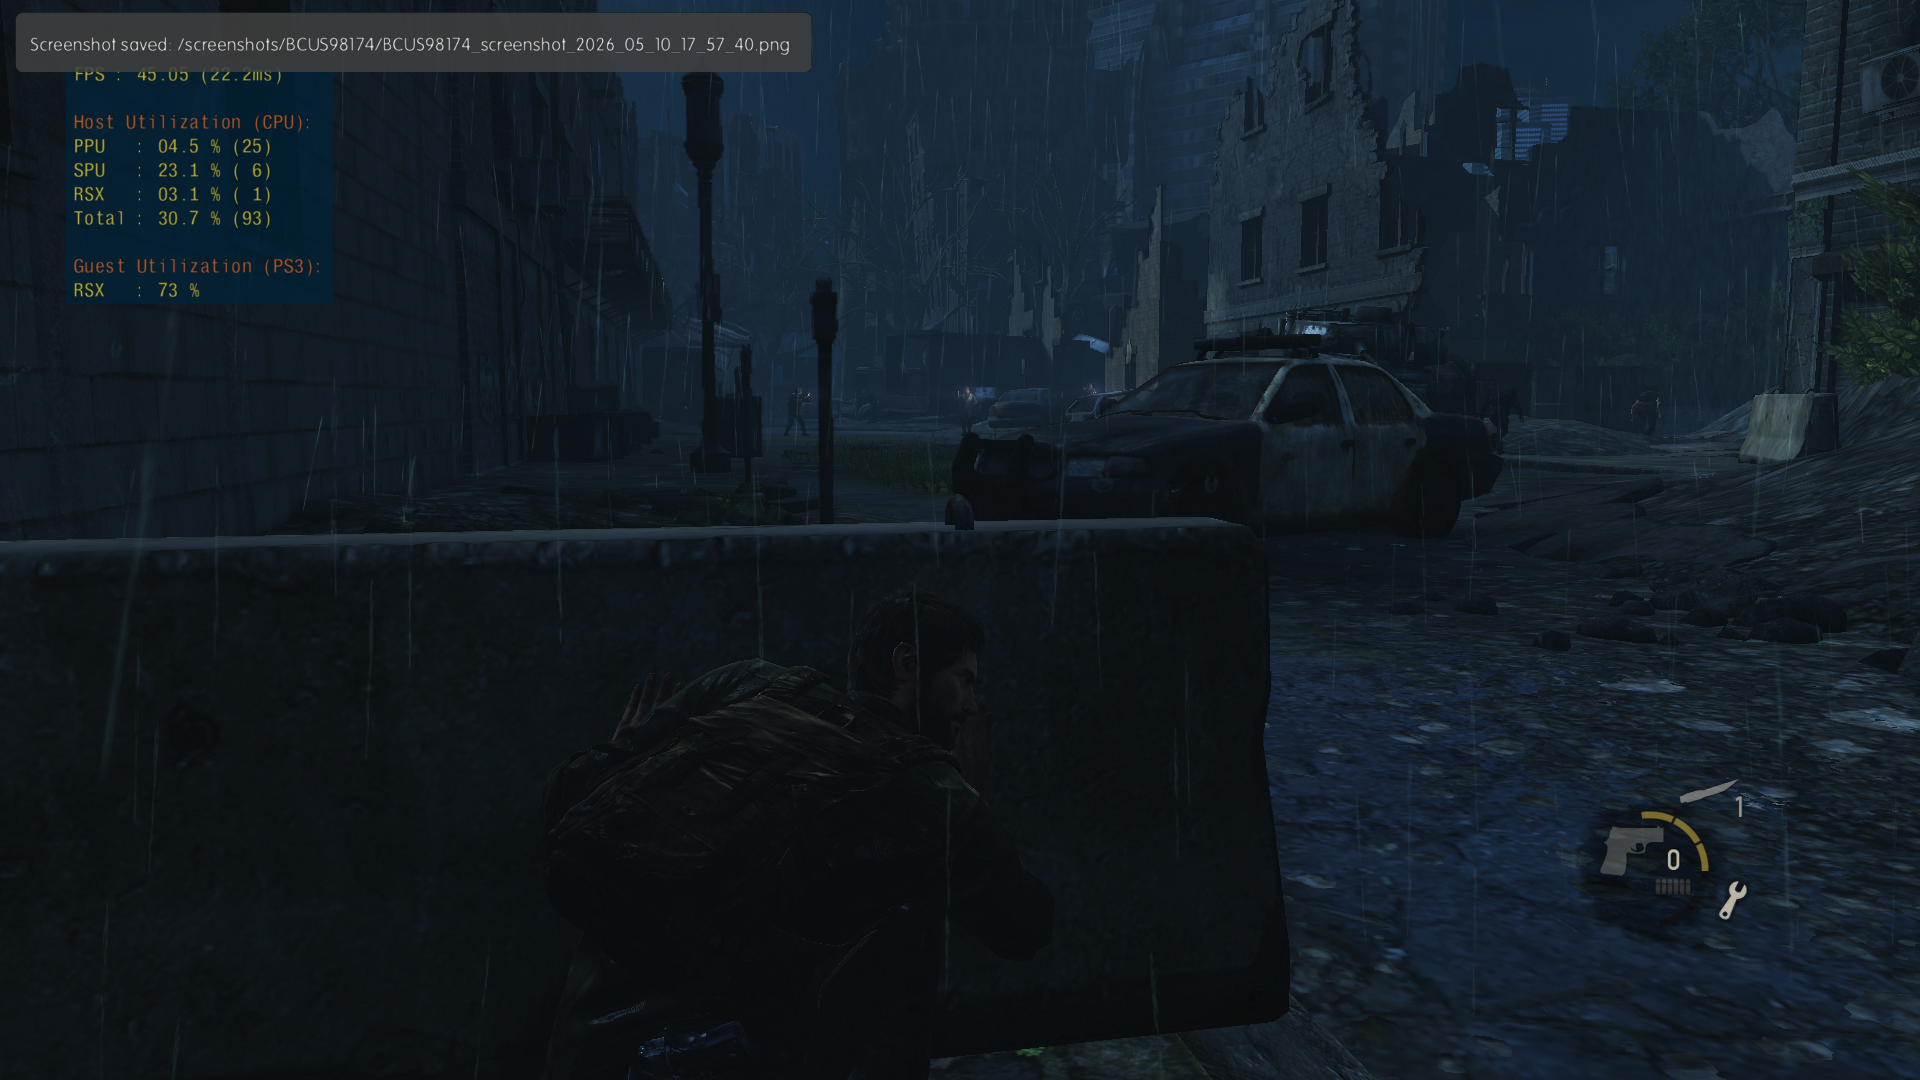
\includegraphics[width=0.9\linewidth]{images/cena1.png}
\caption{Screenshot da cena 1}
\label{fig:c1}
\end{figure}

\begin{figure}[t]
\centering

\includegraphics[width=0.9\linewidth]{images/cena2.png}
\caption{Screenshot da cena 2}
\label{fig:c2}
\end{figure}

O primeiro cenário é parte do capítulo ``Outside'', como na figura 2,
segundo cenário é no capítulo ``Slums'', como na figura 3.

\subsubsection{Instrumentação e
métricas}\label{instrumentauxe7uxe3o-e-muxe9tricas}

O RPCS3 foi instrumentado com um logger personalizado para coleta de
três métricas: frametime (tempo de renderização por quadro) e utilização
dos módulos PPU (Power Processing Unit) e SPU (Synergistic Processing
Units). Os dados foram registrados continuamente durante janelas de 60
segundos por execução.

A modificação principal foi no sistema de monitoramento de performance
do RPCS3, onde um logger contínuo escreve a utilização da SPU, PPU e o
frametime para um arquivo CSV. O logger é ativado através da tecla F2 no
teclado e se desativa automaticamento após 60 segundos. Foi adicionado
um elemento de UI nas configurações de atalho do RPCS3 para remapear a
técla.

\subsubsection{Protocolo experimental}\label{protocolo-experimental}

Para cada combinação de arquitetura de CPU, número de núcleos e cena do
jogo, foram realizadas 5 execuções independentes. Cada execução
consistiu em uma coleta contínua de 60 segundos, totalizando um conjunto
de amostras suficientemente robusto para análise estatística de variação
de desempenho.

No processador Ryzen, as configurações de 6, 8 e 12 núcleos foram
utilizadas. Foram realizados testes em 4 núcleos também, mas a
instabilidade do emulador nessa configuração impediu a coleta de dados
devido a crashes constantes. O processador Intel foi testado com 6
núcleos, sua configuração máxima de núcleos.

Os resultados foram posteriormente agregados para análise comparativa
entre configurações, considerando médias e distribuição de frametime
como principais indicadores de performance.

\section{Conclusão}\label{conclusuxe3o}

Pode ser observado na figura 4 o aumento na variabilidade de utilização
do hardware comparando o múmero diferente de cores. Com 12 cores o
trabalho está espalhado entre vários núcleos, diminuindo variabilidade e
a carga total do sistema. Com 8 cores, a variabilidade aumenta e com 6 a
maior variabilidade é observada. Na figura 6, o aumento do número de
cores espelha a utilização, com a maior variabilidade de quadros vindo
da configuração com 8 núcleos.

Nota-se um grande número de outliers em 8 cores. Também podem ser
notados em 12 cores na figura 6, onde são mais extremos do que em 6
cores. Uma hipótese é que sejam causados pela utilização de dois
complexos de núcleos diferentes. O Ryzen 9 9900X possui dois complexos
no die contendo 6 cores cada, a desabilitação de 4 cores pela BIOS deve
ser feita em 2 cores por complexo, assim sobrando 4 cores em cada. A
comunicação entre os complexos pode estar causando os outlier. Isso pode
ser explorado mais aprofundadamente em um próximo trabalho.

Na figura 5 nota-se que em comparação com o Ryzen 9 9900X, o i5 10400f
tem uma utilização parecida, embora mais variada. Podemos notar na
figura 7 que a mesma quantidade de trabalho não está sendo feita: os
quadros estão sendo gerados em torno de 60 ms no i5 comparado a 25 ms no
Ryzen, menos da metade do tempo para o mesmo número de cores. O aumento
de IPC, a inclusão das instruções AVX512, muito utilizadas no RPCS3, e a
frequência maior do Ryzen 9 9900X podem ser atribuídos a esse aumento de
velocidade.

\begin{figure}

{\centering 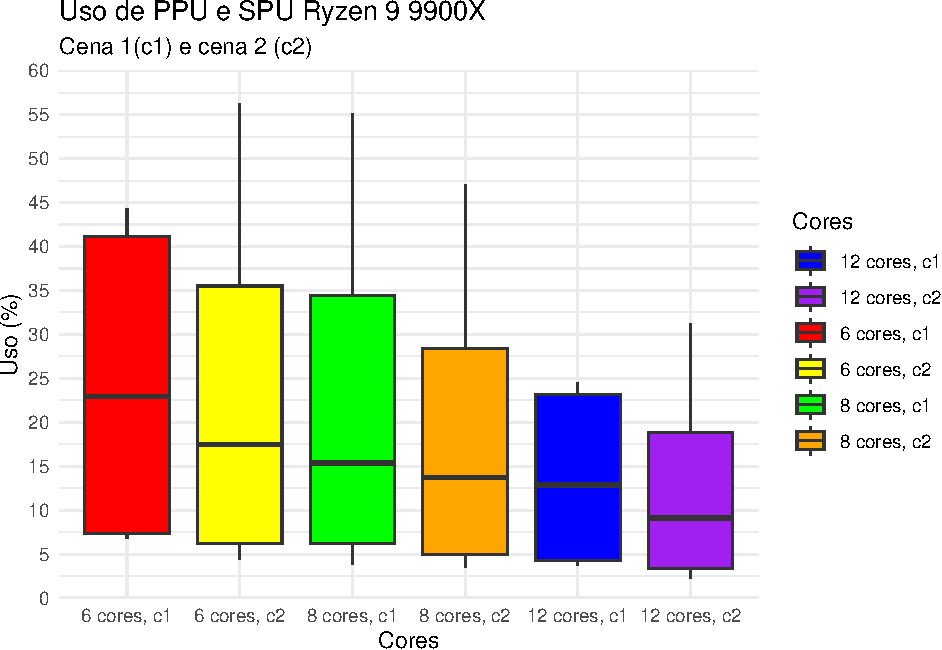
\includegraphics[width=0.85\linewidth]{Report_files/figure-latex/unnamed-chunk-3-1} 

}

\caption{Uso de CPU e PPU para o Ryzen}\label{fig:unnamed-chunk-3}
\end{figure}

\begin{figure}

{\centering 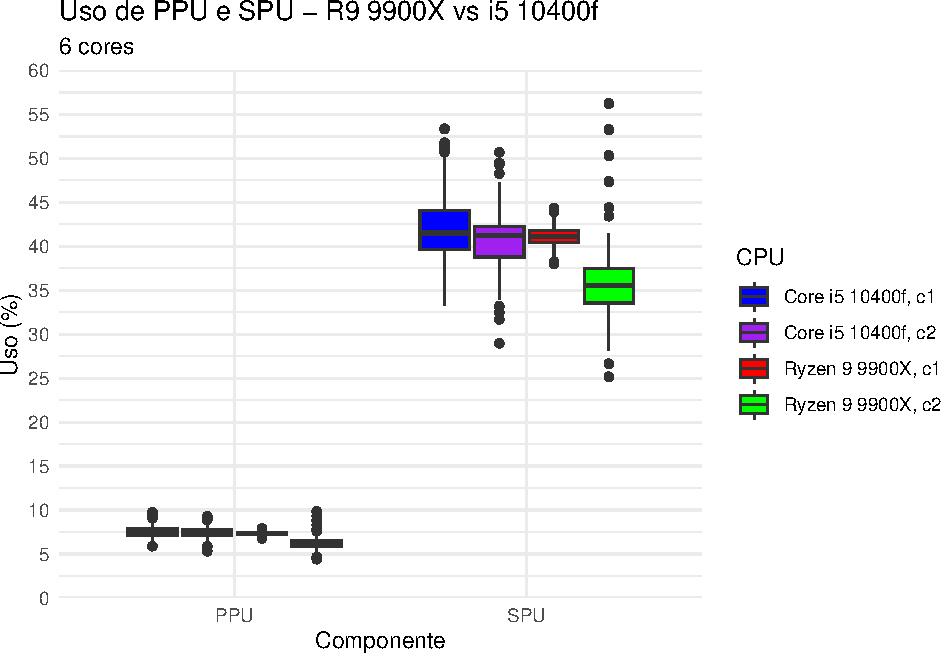
\includegraphics[width=0.85\linewidth]{Report_files/figure-latex/unnamed-chunk-4-1} 

}

\caption{Uso de CPU e PPU comparado entre processadores}\label{fig:unnamed-chunk-4}
\end{figure}

\begin{figure}

{\centering 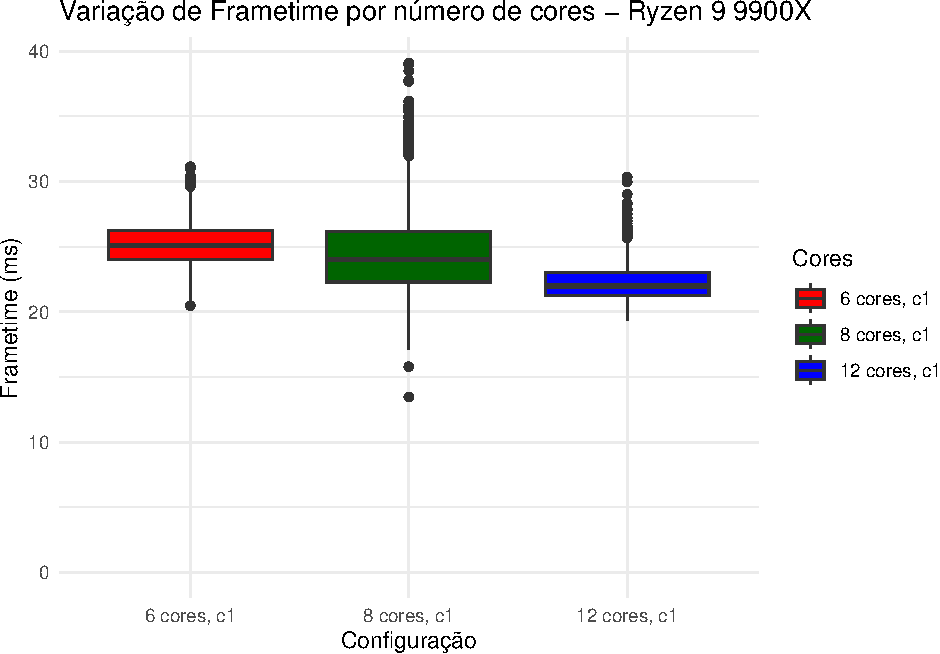
\includegraphics[width=0.7\linewidth]{Report_files/figure-latex/unnamed-chunk-5-1} 

}

\caption{Frametime em ms para configurações diferentes de cores para o Ryzen 9 9900X}\label{fig:unnamed-chunk-5}
\end{figure}

\begin{figure}

{\centering 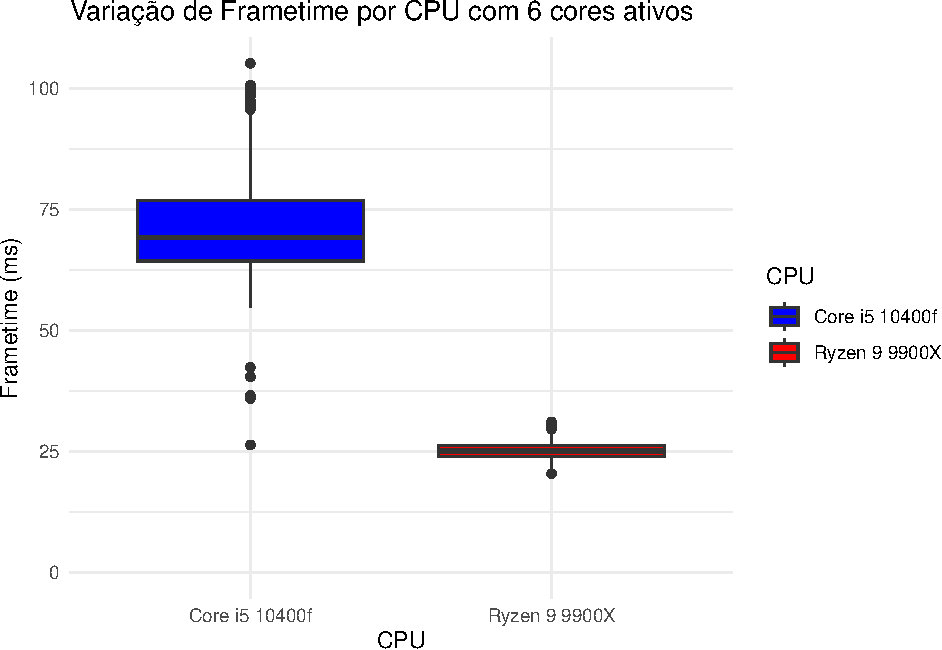
\includegraphics[width=0.7\linewidth]{Report_files/figure-latex/unnamed-chunk-6-1} 

}

\caption{Comparação de frametime em ms para as duas CPUs}\label{fig:unnamed-chunk-6}
\end{figure}

\section{References}\label{references}
\setlength{\parindent}{0in}


\end{document}
